\chapter{Output Feedback}
\label{output_feedback}

Chapter \ref{state_feedback} introduced the concept of reachability. It was shown that it is possible to find 
a state feedback law that gives the desired closed loop eigenvalues provided that the system
is reachable.  Furthermore, we saw how to design controllers using
the system state, $x(t)$, as feedback to out controller. 

However, desigining state feedback controllers preassumes that all the states are measured. For many situations, it
is highly unrealistic to assume that all the states are measured. 

In this section we proceed somehow in a similar vein we can use the output $y(t)$ to modify the dynamics of the system through the use of observers. Furthermore, we will introduce the concept of observability
and show that if a system is observable, it is possible to recover the state
from measurements of the inputs and outputs to the system. We then show how to
design a controller with feedback from the observer state. 




\section{Observability}
\label{observability}

For many situations, it is highly unrealistic to assume that all the states are measured. In this section we
investigate how the state can be estimated by using a mathematical model and a
few measurements. It will be shown that computation of the states can be carried
out by a dynamical system called an \textbf{observer}, see also figure \ref{observer_block_diagram}.


\begin{framed}
\theoremstyle{definition}
\begin{definition}{\textbf{Observability}}
A linear system is \textbf{observable}  if for any $T>0$ it is possible to determine the state of the system $x(T)$ through measurements of $y(t)$ and $u(t)$ on the interval $[0,T]$  $x(T) = x_f$.
\end{definition}
\end{framed}


\begin{framed}
\theoremstyle{remark}
\begin{remark}{\textbf{Nonlinear Systems}}

The definition above holds for nonlinear systems as well, and the results discussed here have extensions to the nonlinear case.
\end{remark}
\end{framed}


Consider again the system

\begin{equation}
\frac{dx}{dt} = Ax + Bu ~~ y = Cx + Du
\end{equation}


where $x\in R^n$ is the state, $u\in R^{p}$ is the input and $y\in R^q$ the measured output.

We wish to estimate the state of the system from its inputs and outputs, as illustrated
in Figure \ref{observer_block_diagram}. In some situations we will assume that there is only one measured
signal, i.e., that the signal $y$ is a scalar and that $C$ is a (row) vector. This signal may
be corrupted by noise $n$, although we shall start by considering the noise-free case.
We write $\hat{x}$ for the state estimate given by the observer.



\begin{figure}[!htb]
\begin{center}
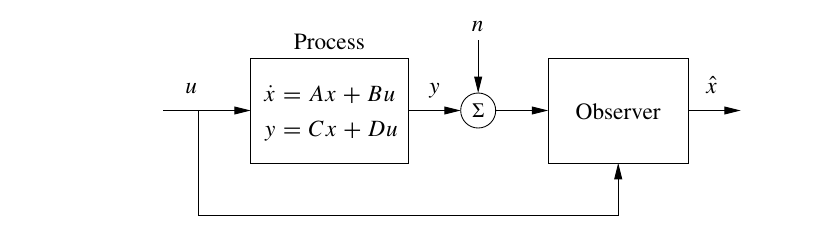
\includegraphics[scale=0.380]{img/output_feedback/observer_block_diagram.jpeg}
\end{center}
\caption{Block diagram for an observer. The observer uses the process measurement $y$
(possibly corrupted by noise $n$) and the input $u$ to estimate the current state of the process,
denoted $\hat{x}$.}
\label{observer_block_diagram}
\end{figure}


The problem of observability is one that has many important applications, even
outside feedback systems. If a system is observable, then there are no hidden dynamics inside it; we can understand everything that is going on through observation (over time) of the inputs and outputs. As we shall see, the problem of observability is of significant practical interest because it will determine if a set of sensors is
sufficient for controlling a system. Sensors combined with a mathematical model
can also be viewed as a virtual sensor that gives information about variables that
are not measured directly. The process of reconciling signals from many sensors
with mathematical models is also called sensor fusion.



\section{Testing for Observability}
\label{test_observability}

When discussing reachability in the last chapter, we neglected the output and focused on the state. Similarly, it is convenient here to initially neglect the input and
focus on the autonomous system



\begin{framed}
\theoremstyle{remark}
\begin{remark}{\textbf{Autonomous System}}

\end{remark}
\end{framed}

\begin{equation}
\frac{dx}{dt} = Ax ~~ y = Cx
\end{equation}

The objective is to understand when it is possible to determine the state from observations of the output. From

\begin{equation}
y = Cx
\end{equation}

we see that the output itself gives us the projection of the state $x$ on vectors that are rows of the matrix $C$. The 
observability problem can  immediately be solved if the matrix $C$ is invertible. If the matrix is not invertible we can take the derivatives and obtain

 
\begin{equation}
\frac{dy}{dt} = C\frac{dx}{dt} = CAx
\end{equation}

From the derivative of the output we thus get the projection of the state on vectors that are rows of the matrix $CA$. Proceeding in this way, we get


\begin{equation}
\begin{bmatrix}
 y \\
 y^{(1)} \\
 \vdots \\
 y^{(n-1)} 
\end{bmatrix} = 
\begin{bmatrix}
 C \\
 CA \\
 \vdots \\
 CA^{n-1} 
\end{bmatrix}x
\end{equation}

We thus find that the state can  be  determined if the observability matrix
 
\begin{equation}
W_o= 
\begin{bmatrix}
 C \\
 CA \\
 \vdots \\
 CA^{n-1} 
\end{bmatrix}
\end{equation}

has $n$ independent rows.  It turns out  that  we  need  not consider any derivatives higher
than $n-1$ (this is an application of the Cayley-Hamilton theorem)
 
\begin{framed}
\theoremstyle{remark}
\begin{remark}{\textbf{System with inputs}}

The calculation can easily be extended to systems with inputs. The state is then
given by a linear combination of inputs and outputs and their higher derivatives.
The observability criterion is unchanged. 
\end{remark}
\end{framed}


\begin{framed}
\theoremstyle{theorem}
\begin{theorem}{Observability rank condition}

A linear system of the form  
\begin{equation}
\frac{dx}{dt} = Ax + Bu ~~ y = Cx + Du \nonumber
\end{equation}

is observable if and only if the observability matrix $W_o$ is full rank.
\end{theorem}
\end{framed}



\section{Observable Canonical Form}
\label{observability_canonical_form}

As in the case of reachability, certain canonical forms will be useful in studying ob-
servability. A linear single-input, single-output state space system is in observable
canonical form if its dynamics are given by

\begin{eqnarray}
\frac{dz}{dt}= 
\begin{bmatrix}
 -\alpha_1 & 1 & 0 & \ldots &  0\\
 -\alpha_2 & 0 & 1 & \ldots &  0 \\
 \vdots \\
-\alpha_{n-1} & 0 & 0 & \ldots &  1 \\
-\alpha_{n} & 0 & 0 & \ldots &  0 \\
\end{bmatrix}z +
\begin{bmatrix}
 b_1 \\
 b_2 \\
 \vdots \\
 b_{n-1}\\
b_{n} 
\end{bmatrix}u \\
y = 
\begin{bmatrix}
 1 & 0 & 0 & \ldots & 0  \\
\end{bmatrix}x + Du
\end{eqnarray}


\begin{framed}
\theoremstyle{remark}
\begin{remark}{\textbf{Observable Canonical Form for Nonlinear Systems}}

The definition can be extended to systems with many inputs; the only difference is
that the vector multiplying u is replaced by a matrix.
\end{remark}
\end{framed}





















\subsection{Reachable Canonical Form}

It is often convenient to change coordinates and write the dynamics of the system in the transformed coordinates

\begin{equation}
z = Tx
\end{equation}

One application of a change of coordinates is to convert a system into a
canonical form in which it is easy to perform certain types of analysis.




The characteristic polynomial for a system in reachable canonical form is given

\begin{equation}
\lambda(s) = s^n +\alpha_1s^{n-1}+ \dots + \alpha_{n-1}s + \alpha_n
\end{equation}

The reachability matrix also has a relatively simple structure:

We now consider the problem of changing coordinates such that the dynamics
of a system can be written in reachable canonical form. Let $A$, $B$ represent the
dynamics of a given system and $\tilde{A}, \tilde{B}$ be the dynamics in reachable canonical form.
Suppose that we wish to transform the original system into reachable canonical
form using a coordinate transformation $z = Tx$. As shown in the last chapter, the
dynamics matrix and the control matrix for the transformed system are


\begin{equation}
\tilde{A} = TAT^{-1}, ~~ \tilde{B} = TB
\end{equation}

The reachability matrix for the transformed system then becomes

\begin{equation}
\tilde{W}_r = \begin{bmatrix}
 \tilde{B} & \tilde{A}\tilde{B} & \ldots & \tilde{A}^{n-1}\tilde{B} 
\end{bmatrix}
\end{equation}

We can transforming each element individually and thus get the reachability matrix fro the transformed system

\begin{equation}
\tilde{W}_r = TW_r
\end{equation}

However, we know that $W_r$ is invertible. Therefore we can solve for the transformation $T$ that takes the system into reachable canonical form:

\begin{equation}
T = \tilde{W}_r W_{r}^{-1}
\end{equation}


\begin{framed}
\theoremstyle{theorem}
\begin{theorem}{Reachable canonical form}

Let $A$ and $B$ be the dynamics and control matrices for a reachable system. Then there exists a transformation

\begin{equation}
z = Tx \nonumber
\end{equation}

such that in the transformed coordinates  the dynamics and control matrices are in the reachable 
canoinical form and the characteristic polynomial for $A$ is given by

\begin{equation}
\text{det}(sI-A) = 0 \nonumber
\end{equation}

\end{theorem}
\end{framed}

One important implication of this theorem is that for any reachable system, we
can assume without loss of generality that the coordinates are chosen such that the
system is in reachable canonical form. This is particularly useful for proofs, as we
shall see later in this chapter. However, for high-order systems, small changes in
the coefficients $a_i$ (that is the coefficients of the characteristic polynomial) can give large changes in the eigenvalues. Hence, the reachable canonical form is not always well conditioned and must be used with some care.


\section{Stabilization by State Feedback}

In this section, we will assume that the
system to be controlled is described by a linear state model and has a single input
(for simplicity). The feedback control law will be developed step by step using a
single idea: the positioning of closed loop eigenvalues in desired locations.

Figure \ref{state_feedback_sys_II} has already been shown at the begining of this chapter. It shows a diagram of a typical control system using state feedback.


\begin{figure}[!htb]
\begin{center}
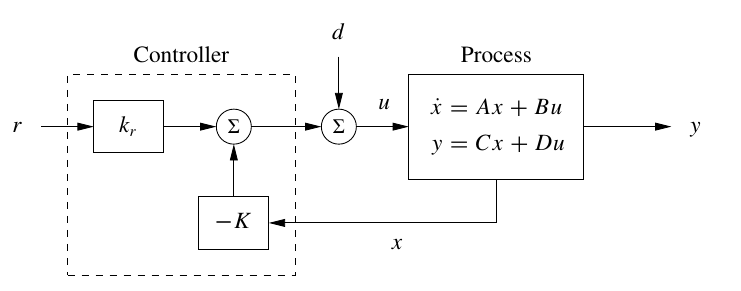
\includegraphics[scale=0.280]{img/state_feedback/state_feedback_sys.jpeg}
\end{center}
\caption{A feedback control system with state feedback. The controller uses the system
state $x$ and the reference input $r$ to command the process through its input $u$. We model
disturbances via the additive input $d$.}
\label{state_feedback_sys_II}
\end{figure}

The full system consists of the process dynamics, which we take to be linear, the controller
elements $K$ and $k_r$ , the reference input (or command signal) $r$ and process disturbances $d$. The goal of the feedback controller is to regulate the output of the system $y$ such that it tracks the reference input in the presence of disturbances and also uncertainty in the process dynamics.

An important element of the control design is the performance specification.
The simplest performance specification is that of stability: in the absence of any
disturbances, we would like the equilibrium point of the system to be asymptotically
stable. More sophisticated performance specifications typically involve giving desired properties of the step or frequency response of the system, such as specifying the desired rise time, overshoot and settling time of the step response. Finally, we are often concerned with the disturbance attenuation properties of the system: to
what extent can we experience disturbance inputs $d$ and still hold the output $y$ near the desired value?

Consider a system described by the linear differential equation



\begin{equation}
\frac{dx}{dt} = Ax + Bu ~~ y = Cx + Du
\end{equation}






